% !TEX root = applied-math.tex

\chapter{Fourier Series}   \label{ch:fourier:series}
 
\section{Properties of Functions}

In section \ref{sect:inner:product}, we reviewed inner product spaces and saw orthonormal sets of vectors (both in $\mathbb{R}^3$ as well as polynomials).  In this section, we will examine another set of functions, sines and cosines that are orthogonal.  First, let's see a short review of periodic functions.  

\subsection{Periodic Functions}


\begin{definition}
A function is \textbf{periodic with period $p$} if
% 
\begin{align*}
f(t) & = f(t+p)
\end{align*}
for all $t$ in the domain of $f$.  The smallest value of $p>0$ that makes this true is called the \textbf{period} of the function.  
\end{definition}

\begin{example}
Show that $f(t) = \sin t$ is periodic with period $2\pi$.  

\solution

\begin{align*}
f(t+2\pi) & = \sin (t + 2 \pi) = \sin t \cos 2\pi + \sin 2\pi \cos t = \sin t 
\end{align*}
\end{example}

\begin{example}
What is the period of the function $f(t) = \cos kt$.

\solution

We know that the period of $\cos t$ is also the same as $\sin t$ or $2\pi$.  If we let $u=kt$, then $f(u)=\cos u$ has period $p=2\pi$ since it is the smallest value of $p$ such that $f(u)=f(u+p)$ for all $u$.  The function $f(t)$ would then had period $p=2\pi/k$, since $t=u/k$.  

\end{example}

The standard period functions that we will be using in this text are the sine and cosine function.  We review here a few convenient identities with these functions and the complex exponential.  From Euler's formula,
%
\begin{align*}
e^{i \theta} & = \cos \theta  + i \sin \theta
\end{align*}
we can then write sine and cosine in terms of $e^{i \theta}$
%
\begin{align*}
\sin \theta & = \frac{e^{i \theta}- e^{-i \theta}}{2i} & \cos \theta & = \frac{e^{i \theta} + e^{-i \theta}}{2} 
\end{align*}

Euler's formula also leads to the following:

\begin{Boxed*}
\noindent{}\textbf{The Most Interesting Equation in Mathematics}

\begin{align} 
e^{i\pi} + 1 = 0  \label{eq:e:to:the:i:pi}
\end{align}
\end{Boxed*}
%
and this is often called the most interesting equation in mathematics because it arguably contains the 5 most important mathematical constants: 0, 1, $e$, $i$, $\pi$.  




\begin{lemma} \label{lem:int:complex:exp}
If $k \in \mathbb{Z}$,  and  $x_0 \in \mathbb{R}$  then 
%
\begin{align*}
\int_{x_0}^{x_0 + 2\pi} e^{i kx} \, dx & = \begin{cases}
2\pi & k = 0, \\
0 & \text{otherwise}.
\end{cases}
\end{align*}
\end{lemma}

\begin{proof}

If $k=0$, then the integral is of the constant function 1 over a interval of length $2\pi$, so the lemma holds,  If $k \neq 0$, 

\begin{align*}
\int_{x_0}^{x_0 + 2\pi} e^{i kx} \, dx & = \frac{e^{i k x}}{i k} \biggr \vert_{x_0} ^{x_0 + 2\pi}   \\
& = \frac{1}{ik} \bigl( e^{ik(x_0+2\pi)} - e^{ikx_0} \bigr) \\
& = \frac{1}{ik} e^{ikx_0} (e^{2\pi i k} -1 ) \\
& = \frac{1}{ik} e^{ikx_0} ( (e^{i\pi})^{2k} -1 ) = 0 
\end{align*}
because $e^{i\pi}=-1$ from (\ref{eq:e:to:the:i:pi}),  but this is raised to an even power so $(e^{i\pi})^{2k}=1$ 

\end{proof}

\subsection{One-Side Limits and Derivatives; Piecewise Continuous Functions}

As we will see, the notion of a piecewise continuous function is a function that is continuous on subintervals.  However, there are some technical details that we need before a formal definition.  

\begin{definition} \index{left-hand limit}\index{right-hand limit}
A function $f$ has a \textbf{left-hand limit} at $x=x_0$ if 
%
\begin{align*}
f(x_0^-) & = \lim_{x \rightarrow x_0^-} f(x) 
\end{align*}
exists.  In addition, a function $f$ has a \textbf{right-hand limit} at $x=x_0$ if 
%
\begin{align*}
f(x_0^+) & = \lim_{x \rightarrow x_0^-} f(x) 
\end{align*}
exists.  
\end{definition}

If one is talking about either a left- or right-handed limit, these are typically called one-sided limits.  
\index{one-sided limit}
\begin{definition} \index{left-hand derivative}\index{right-hand derivative}
A function $f$ has a \textbf{left-hand derivative} at $x=x_0$ if 
% 
\begin{align*}
f'(x_0^-) & = \lim_{h \rightarrow 0^-} \frac{f(x_0+h)-f(x)}{h} 
\end{align*} exists.   Similarly, a function $f$ has a \textbf{right-hand derivative} at $x=x_0$ if 
% 
\begin{align*}
f'(x_0^+) & = \lim_{h \rightarrow 0^+} \frac{f(x_0+h)-f(x)}{h} 
\end{align*} exists.  
\end{definition}

If one is talking about either a left- or right-handed derivative, these are typically called one-sided derivatives. \index{one-sided derivative}

\begin{definition}
A function $f$ is \textbf{piecewise continuous} on an interval $[a,b]$ if $f$ is continuous on all $x \in [a,b]$ except for a finite number of points $x_i$.   In addition for all $x_i$, $f(x_i^+)$ and $f(x_i^-)$ exist.  
\index{piecewise continuous}\index{function!piecewise continuous}
\end{definition}

\begin{example} \label{ex:piecewise:cont:function}
The following function is piecewise continuous on $[-1,1]$
% 
\begin{align*}
f(x) & = \begin{cases}
1 & -1 \leq x < 0 \\
x & 0 \leq x < 1/2 \\
1-x^2 & 1/2 \leq x \leq 1
\end{cases}
\end{align*}

Also, the graph of piecewise functions are helpful.  These are found by finding the graphs of $f$ on each given interval. The graph of $f$ is shown below. 

\begin{center}
\begin{tikzpicture}[scale=2]
\draw[->] (-1.5,0) -- (1.5,0) node [above right] {$x$};
\draw[->] (0,-1.5) -- (0,1.5) node [above right] {$y$}; 


% this draws all non fractional multiples of pi


\draw[*-o](-1.05,1) -- (0.05,1);
\draw[*-o](-0.05,0) -- (0.55,0.5);
\draw[*-*] plot [domain=0.45:1.05] (\x,{1-\x*\x});

\foreach \x/\val in {0.5/\frac{1}{2},1/1,-0.5/-\frac{1}{2},-1/-1}
\draw ({\x},0.1) -- ({\x},-0.1) node [below] {$\val$}; 

\foreach \y in {-1,1} \draw (-0.1,\y) -- (0.1,\y) node [right] {\y};

\end{tikzpicture}
\end{center}

In addition, we need to show that all of the one-sided limits exist.  

\begin{align*}
\lim_{x \rightarrow 0^-} f(x) & = 1 & \lim_{x \rightarrow 0^+} f(x) & = 0 \\
\lim_{x \rightarrow \frac{1}{2}^-} f(x) & = \frac{1}{2} & \lim_{x \rightarrow \frac{1}{2}^+} f(x) & = \frac{3}{4} \\
\end{align*}
%
And since the function is continuous at all points except at 0 and 1/2, but the one-sided limits are finite here, then the function $f$ is piecewise continuous.  

\end{example}

\phantom{hi}

\begin{example}
Find both the left- and right-handed derivatives of the function defined in example \ref{ex:piecewise:cont:function} at $x=0$ and $x=1/2$.  

\solution

First, consider the derivative of the function 
\begin{align*}
f'(x) & = \begin{cases}
0 & -1 < x < 0 \\
1 & 0 < x < 1/2 \\
-2x & 1/2 < x < 1
\end{cases}
\end{align*}
where the equality parts of the derivative have been removed (and explained later). 

Since
%
\begin{align*}
\lim_{x \rightarrow 0^{-}} f'(x) & = 0 & \lim_{x \rightarrow 0^+} & = 1 \\
\lim_{x \rightarrow \frac{1}{2}^{-}} f'(x) & = 1 & \lim_{x \rightarrow \frac{1}{2}^+} & = -1 \\
\end{align*}
then the left-handed derivative at 0 is 0, the right-handed derivative of $f$ at 1, the left-handed derivative at 1/2 is 1 and the right-handed derivative of $f$ at 1/2 is -1.  

\end{example}


\begin{example}
Show that $f(x)=1/x$ is not a piecewise continuous function on $[-1,1]$.  

\solution

The problem in this function on the interval $[-1,1]$ is at $x=0$.  Also
%
\begin{align*}
\lim_{x \rightarrow 0^-} f(x) & = -\infty & \lim_{x \rightarrow 0^+} f(x) & = \infty
\end{align*}
and since the one-sided limits do not exist, $f$ is not piecewise continuous on $[-1,1]$. 

\end{example}

\subsection{Odd and Even Functions} 

\begin{definition}
A function $f(x)$ is an \textbf{odd function} if $f(-x) = -f(x)$ for all $x$ in its domain.  \index{odd function}\index{function!odd}
\end{definition}

Note: recall that an odd function is symmetric about the origin, meaning that if the graph of $f$ is rotated a half circle about the origin, that one gets the graph back.  

\begin{definition}
A function $f(x)$ is an \textbf{even function} if $f(-x)=f(x)$ for all $x$ in its domain.   \index{even function}\index{function!even}
\end{definition}

Recall that an even function is symmetric about the $y$-axis.  This means that if the graph is reflected over the $y$-axis that one gets the same graph upon the reflection. 



\begin{example}
Here's a list of a few functions that are odd or even (without showing details): 
\begin{itemize}
\item The following functions are odd: $x, x^3, x^5, \sin x, \tan x$ 

\item The following functions are even: $1,x^2,x^4, \cos x$.  
\end{itemize}

\end{example}

The following theorem is helpful for finding whether or not products of functions are odd or even.

\begin{theorem}  ~~

\begin{itemize}
\item The product of two odd functions is even.  
\item The product of two even functions is even. 
\item The product of an even and an odd function is odd. 
\end{itemize}

\end{theorem}

\begin{lemma}
The derivative of an even function is odd.  The derivative of an odd function is even. 
\end{lemma}

\begin{proof}
Let $f$ be an even function, then $f(-x) = f(x)$ for all $x$. 
% 
\begin{align*}
\frac{d}{dx} f(x) & = \frac{d}{dx} f(-x) = -\frac{df(-x)}{dx}
\end{align*}
by the chain rule.   And the proof that the derivative of an odd function is similar. 
\end{proof}

And as a corollary, antiderivatives work in the same way.  



\begin{corollary}
~
\begin{itemize}
\item Let $f$ be an odd function.  Any antiderivative of $f$ is even.  
\item Let $g$ be an even function and $G$ be its antiderivative.  The antiderivative $G(x)+C$ such that $C=-G(0)$ is odd.  
\end{itemize}

\end{corollary}



\begin{theorem} Let $f$ be a piecewise continuous function on the interval $[-a,a]$ for $a>0$.  

\begin{itemize}
\item If $f$ is an odd function then 
% 
\begin{align*}
\int_{-a}^a f(x) \, dx & = 0 
\end{align*}
\item If $f$ is an even function then 
% 
\begin{align*}
\int_{-a}^a f(x) \, dx & = 2 \int_{0}^a f(x) \, dx 
\end{align*}
\end{itemize}
\end{theorem}

\begin{proof}
First, examine the first statement.  Let $F(x)$ be an antiderivative of $f(x)$, an odd function.  The function $F(x)$ can be written as $F(x)=G(x)+C$ where $G(x)$ is an even function. 
% 
\begin{align}
\int_{-a}^a f(x) \,dx & = G(x) + C \biggl\vert_{-a}^a = G(-a)+C - (G(a)+C) = 0 
\end{align}
since $G(x)$ is even.   The proof of the second statement is similar.  
\end{proof}





\subsection{Tabular Integration}

A very handy formula for many integrations in this section is called \textbf{tabular integration},\index{tabular integration} which is just a recursive version of integration by parts that works well for integrals of a certain type.  Before we show this, recall that the integration by parts formula is
%
\begin{align*}
\int u \, dv & = uv - \int v \, du
\end{align*}
and integration by parts is helpful for rewriting one integral (on the left) in terms of a second integral (on the right) and generally it is used to create a simpler integral. The next example shows a standard integration done with integration by parts. 

\begin{example}
Find 
%
\begin{align*}
\int x e^x \, dx 
\end{align*}

\solution

In this case, we'll let $u= x$ and $dv = e^x \, dx$, finding the differential $u$ results in $du=dx$ and finding an antiderivative of $dv$ results in $v= e^x$, so using integration by parts to get
%
\begin{align*}
\int x e^x \, dx & = x e^x - \int e^x \, dx  \intertext{and finding the antiderivative of $e^x$,}
& = x e^x - e^x + C 
\end{align*}
\end{example}

This example shows that in order to integrate with the by parts formula, one must replace one integral with another.  In more difficult examples, this may need to be done multiple times until the resulting integral is able to be done without by parts.  This is the case when tabular integration is useful.  

\phantom{hi}

\begin{Boxed*}
The technique of \textbf{tabular integration} applied to 
%
\begin{align*}
\int f(x) g(x) \, dx 
\end{align*}
where there exists an $n$ such that $f^{(n)}(x)=0$, that is eventually the derivative of $f(x)$ is 0.  Creates a table of three columns with 

\begin{enumerate}[label=\textbf{Column \arabic*:},itemindent=0.5in]
\item The function $f(x)$ and its derivatives until you reach zero.
\item The signs $+$ and $-$, starting with $+$ and alternating signs. 
\item The function $g(x)$ and its antiderivatives.

\end{enumerate}
For columns 2 and 3, continue until you reach the same row as the 0 in the first column. 

To find the antiderivative, draw arrows from each function in the first column, to a function in the third column one row below.  The result is the sum of the product of each pair of functions connected by the arrows with the sign of that above the given arrow.  
\end{Boxed*}

This is best seen with a couple of examples.  

\begin{example}
Find 
%
\begin{align*}
\int x^3 e^x \, dx
\end{align*}
using tabular integration. 

\solution

First, we will build the table:

\begin{center}
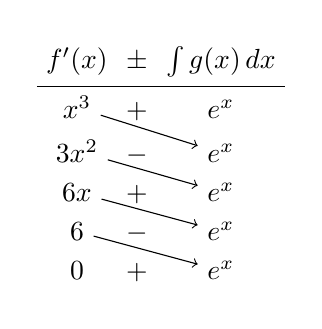
\begin{tikzpicture}[every node/.style={anchor=base}]
  \matrix
  {
    \node (f1){$f'(x)$}; & \node{$\pm$}; & \node (g1) {$\int g(x) \, dx$}; \\ \hline
    \node (f2){$x^3$}; & \node {$+$}; & \node (g2) {$e^x$}; \\
    \node (f3) {$3x^2$}; & \node {$-$}; & \node (g3) {$e^x$}; \\
    \node (f4){$6x$}; & \node {$+$}; & \node (g4) {$e^x$}; \\
    \node (f5){$6$}; & \node {$-$}; & \node (g5) {$e^x$}; \\
    \node (f6){$0$}; & \node {$+$}; & \node (g6) {$e^x$}; \\
  };
    \draw[->] (f2)--(g3); 
    \draw[->] (f3)--(g4); 
    \draw[->] (f4)--(g5); 
    \draw[->] (f5)--(g6); 
\end{tikzpicture}
\end{center}
and then read off the result which is the product of terms connected by the arrows with the sign above each arrow. 

\begin{align*}
\int x^3 e^x \, dx & = x^3 e^x - 3x^2 e^x + 6x e^x - 6 e^x + C 
\end{align*}
and don't forget the $C$ for an indefinite integral.  
\end{example}

And the following is an example that is similar as we will see below:
%
\begin{example}
Find 
\begin{align*}
\int_0^{\pi} x^2 \cos 2x \, dx 
\end{align*}
using tabular integration. 

\solution

First, we will build the table:

\begin{center}
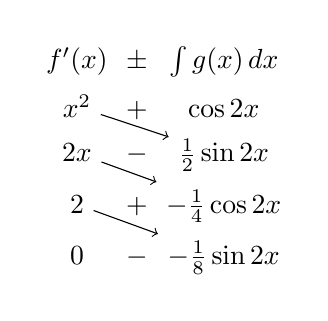
\begin{tikzpicture}[every node/.style={anchor=base}]
  \matrix
  {
    \node (f1){$f'(x)$}; & \node{$\pm$}; & \node (g1) {$\int g(x) \, dx$}; \\
    \node (f2){$x^2$}; & \node {$+$}; & \node (g2) {$\cos 2x $}; \\
    \node (f3) {$2x$}; & \node {$-$}; & \node (g3) {$\frac{1}{2} \sin 2x$}; \\
    \node (f4){$2$}; & \node {$+$}; & \node (g4) {$-\frac{1}{4} \cos 2x$}; \\
    \node (f5){$0$}; & \node {$-$}; & \node (g5) {$-\frac{1}{8} \sin 2x $}; \\
  };
    \draw[->] (f2)--(g3); 
    \draw[->] (f3)--(g4); 
    \draw[->] (f4)--(g5); 
\end{tikzpicture}
\end{center}
and then read off the result which is the product of terms connected by the arrows with the sign above each arrow. 

\begin{align*}
\int_0^{\pi} x^2 \cos 2x \, dx & = \biggl( \frac{x^2}{2} \sin 2x + \frac{x}{2} \cos 2x - \frac{1}{4} \sin 2x \biggr) \biggr \vert_{0}^{\pi} \\
& = \biggl(\frac{\pi^2}{2} \sin 2\pi + \frac{\pi}{2} \cos 2\pi - \frac{1}{4} \sin 2\pi \biggr) \\
& \qquad - \biggl(0 + 0 - \frac{1}{4} \sin 0 \biggr) \\
& = \frac{\pi}{2} 
\end{align*}

\end{example}



\subsection{Inner Products of Functions}

As we saw in section \ref{sect:inner:product}, the inner product\index{functions!inner product of} of two functions can be defined using the integral.  In this section, we consider functions that are piecewise continuous on $[a,b]$ and 
% 
\begin{align*}
\langle f, g \rangle & = \int_a^b f(x) g(x) \, dx 
\end{align*}

In the standard way, the norm of $f$\index{function!norm} is defined as 
% 
\begin{align*}
|| f || & = \langle f, f \rangle^{1/2} = \biggl( \int_a^b f^2(x) \, dx \biggr)^{1/2} 
\end{align*}


\begin{definition}
An infinite set of continuous function $\{f_1,f_2, \ldots\}$ is said to be \textbf{orthogonal on $[a,b]$} if\\ $\langle f_n, f_m \rangle =0$ for all $n,m$, $n \neq m$.  If in addition, $||f_n||=1$ for all $n$, the set is said to be \textbf{orthonormal}.  \index{orthogonal}\index{functions!orthogonal set}\index{orthonormal}\index{functions!orthonormal}
\end{definition}

In the next couple of examples, we examine a couple of the most important orthogonal and orthonormal sets of functions.  


\begin{example}
Show that $f_n(x) = \sin nx$ for $n=1,2,3,\ldots$ form an orthogonal set on $[-\pi,\pi]$.  

\solution

In this case, we will expand on the example \ref{ex:orthog:set} and use the handy alternative definition of the sine function.  Find the inner product if $n \neq m$, 
%
\begin{align*}
\langle f_n, f_m \rangle & = \int_{-\pi}^{\pi} \sin nx \sin mx \, dx \\
& = \int_{-\pi}^{\pi} \frac{e^{i n x} - e^{-i n x}}{2i}\frac{e^{i mx} - e^{-i m x}}{2i} \, dx  \\
& = -\frac{1}{4} \int_{-\pi}^{\pi} \bigl( e^{i(m+n)x} - e^{i(m-n) x}- e^{i(n-m) x} + e^{-i(m+n) x} \bigr) \, dx \intertext{Using Lemma \ref{lem:int:complex:exp}}
& = 0 
\end{align*}
\end{example}

\begin{example} \label{ex:trig:ortho:set}
Show that the set of functions 
% 
\begin{align*}
\biggl\{ \frac{1}{\sqrt{2\pi}}, \frac{1}{\sqrt{\pi}} \cos x , \frac{1}{\sqrt{\pi}} \sin x, \frac{1}{\sqrt{\pi}} \cos 2x, \frac{1}{\sqrt{\pi}} \sin 2x, \ldots  \biggr\}
\end{align*}
for an orthonormal set on $[-\pi,\pi]$.  


\solution

We showed above that $\langle \sin mx, \sin nx \rangle=0$ for all $m,n$ when $m \neq n$.   Therefore $\langle (\sin mx)/\sqrt{\pi}, (\sin nx)/\sqrt{\pi} \rangle$.   For simpler notation let
%
\begin{align*}
s_n(x) & = \frac{1}{\sqrt{\pi}}\sin n x, \qquad \text{n>0} \\
c_n(x) & = \begin{cases} 
\frac{1}{\sqrt{2\pi}} & n = 0, \\
\frac{1}{\sqrt{\pi}} \cos nx  & n>0,
\end{cases}
\end{align*}

First, we will show that $\langle s_m (x), c_n(x) \rangle=0$ for all $n, m>0$.  
\begin{align*}
\langle s_m (x), c_n (x) \rangle & = 
\biggl\langle \frac{1}{\sqrt{\pi}}\sin mx, \frac{1}{\sqrt{\pi}}\cos nx  \biggr\rangle \\
&  = \frac{1}{\pi} \int_{-\pi}^{\pi} \sin mx  \cos nx \,dx \\
& = \frac{1}{\pi} \int_{-\pi}^{\pi} \frac{e^{imx} - e^{-imx}}{2i} \frac{e^{inx}+e^{-inx}}{2} \, dx \\
& = \frac{1}{4i\pi} \int_{-\pi}^{\pi} \bigl( e^{i(m+n)x}-e^{i(n-m)x}+e^{i(m-n)x}-e^{-i(m+n)x} \bigr) \, dx  \\ &  = 0 
\end{align*}
since each integral is zero from Lemma \ref{lem:int:complex:exp}.  Next, we will show that\\ $\langle c_m(x), c_n(x) \rangle = 0$ for all $n,m >0$ such that $n \neq m$. 

\begin{align*}
\langle c_m (x), c_n (x) \rangle & = 
\biggl\langle \frac{1}{\sqrt{\pi}}\cos mx, \frac{1}{\sqrt{\pi}}\cos nx  \biggr\rangle \\
&  = \frac{1}{\pi} \int_{-\pi}^{\pi} \cos mx  \cos nx \,dx \\
& = \frac{1}{\pi} \int_{-\pi}^{\pi} \frac{e^{imx} + e^{-imx}}{2} \frac{e^{inx}+e^{-inx}}{2} \, dx \\
& = \frac{1}{4\pi} \int_{-\pi}^{\pi} \bigl( e^{i(m+n)x} +e^{i(n-m)x}+e^{i(m-n)x}+e^{-i(m+n)x} \bigr) \, dx   \\ &= 0 
\end{align*}
because again each integral is zero from Lemma \ref{lem:int:complex:exp}. 


Lastly, we need to show that the norm of each of the functions is 1.  
\begin{align*}
\langle c_0, c_0 \rangle & = \int_{-\pi}^{\pi} \biggl(\frac{1}{\sqrt{2\pi}} \biggr)^2 \, dx = 1 , \\
\langle c_n, c_n \rangle & = 
\frac{1}{\pi} \int_{-\pi}^{\pi} \cos^2 nx \, dx \\
& = \frac{1}{\pi} \int_{-\pi}^{\pi} \biggl( \frac{e^{inx} + e^{-inx}}{2} \biggr)^2 \, dx \\
& = \frac{1}{4\pi} \int_{-\pi}^{\pi} \bigl( e^{2inx} + 2 + e^{-2inx} \bigr) \, dx 
\intertext{and the integrals of the first and third terms are zero from Lemma \ref{lem:int:complex:exp}. }
& = \frac{1}{4\pi} \int_{-\pi}^{\pi}  2 \, dx  = 1 \\
\langle s_n, s_n \rangle & = 
\frac{1}{\pi} \int_{-\pi}^{\pi} \sin^2 nx \, dx \\
& = \frac{1}{\pi} \int_{-\pi}^{\pi} \biggl( \frac{e^{inx} - e^{-inx}}{2i} \biggr)^2 \, dx \\
& = \frac{1}{(2i)^2\pi} \int_{-\pi}^{\pi} \bigl( e^{2inx} - 2 + e^{-2inx} \bigr) \, dx 
\intertext{and the integrals of the first and third terms are zero from Lemma \ref{lem:int:complex:exp}. }
& = \frac{1}{-4\pi} \int_{-\pi}^{\pi}  -2 \, dx  = 1 \\
\end{align*}

This shows that the set of functions given above is an orthonormal set of functions.  
\end{example}


\section{Fourier Series}


An infinite series of the form:
%
\begin{align*}
 a_0 + \sum_{n=1}^{\infty} (a_n \cos n x + b_n \sin nx) 
\end{align*}
is called the \textbf{trigonometric series}. \index{trigonometric series} 


The trigonometric series is periodic with period at most $2\pi$.  Consider the terms $\cos x$ and $\sin x$, which each have period $2\pi$.  All other functions have period $2\pi/n$, which are also periodic with period $2\pi$, but their fundamental period is $2\pi/n$.    


\begin{definition}
Let $f(x)$ be periodic of period $2\pi$ and be piecewise continuous in $[-\pi,\pi]$.  Suppose $f(x)$ can be written as a trigonometric series.  Then it is called a \textbf{Fourier Series}\index{Fourier Series} for $f(x)$.  The constants $a_n$ and $b_n$ are called the \textbf{Fourier Coefficients}\index{Fourier Coefficients} of $f(x)$ and are given by the Euler formulas:



\begin{align}
a_0 & = \frac{1}{2\pi} \langle f(x), 1 \rangle = \frac{1}{2\pi} \int_{-\pi}^{\pi} f(x) \, dx \label{eq:fourier:coeff:a0}\\
a_n & = \frac{1}{\pi} \langle f(x), \cos n x \rangle = \frac{1}{\pi} \int_{-\pi}^{\pi} f(x) \cos nx \, dx \label{eq:fourier:coeff:an}\\
b_n & = \frac{1}{\pi} \langle f(x), \sin nx \rangle = \frac{1}{\pi} \int_{-\pi}^{\pi} f(x) \sin nx \, dx \label{eq:fourier:coeff:bn}\\
\end{align}
\end{definition}

In this section, we're going to write period functions as Fourier Series.  This is possible due to the following theorem. 

\begin{theorem} \label{thm:fourier:series}
Let $f$ be a continuous function that is periodic with period $2\pi$.  Then $f$ can be written as a trigonometric series or 
\begin{align}
f(x) & = a_0 + \sum_{n=1}^{\infty} (a_n \cos n x + b_n \sin nx).   \label{eq:trig:series} 
\end{align}
\end{theorem}


\begin{proof}

In this proof, we will take the inner product of $f$ with each element in the set from Example \ref{ex:trig:ortho:set}.   We will start with the constant function and use (\ref{eq:trig:series}).  

\begin{align*}
\biggl\langle \frac{1}{\sqrt{2\pi}}, f(x) \biggr\rangle & = \biggl\langle \frac{1}{\sqrt{2\pi}},  a_0 + \sum_{n=1}^{\infty} (a_n \cos n x + b_n \sin nx)  \biggr\rangle   \\
 \frac{1}{\sqrt{2\pi}} \langle 1, f(x) \rangle & = \frac{1}{\sqrt{2\pi}} \biggl(\langle a_0,1 \rangle + \sum_{n=1}^{\infty} a_n \langle \cos nx, 1 \rangle + b_n \langle \sin nx , 1 \rangle  \biggr)  
\intertext{since the inner product of 1 with the trig functions are 0} 
& = \frac{a_0}{\sqrt{2\pi}} \langle 1, 1 \rangle
\end{align*}
and solving for $a_0$, 
% 
\begin{align*}
a_ 0 & = \frac{\langle f(x),1 \rangle}{\langle 1,1 \rangle}  = \frac{1}{2\pi} \int_{-\pi}^{\pi} f(x) \, dx 
\end{align*}

Next, take the inner product of (\ref{eq:trig:series}) with $\frac{1}{\sqrt{\pi}}\cos nx$. 

\begin{align*}
\biggl\langle \frac{1}{\sqrt{\pi}}\cos nx ,f(x) \biggr \rangle & = \biggl\langle \frac{1}{\sqrt{\pi}}\cos nx,  a_0 + \sum_{m=1}^{\infty} (a_m \cos m x + b_m \sin mx)  \biggr\rangle  \\
\frac{1}{\sqrt{\pi}} \langle \cos nx, f(x) \rangle & = \frac{1}{\sqrt{\pi}} \biggl(a_0 \langle 1, \cos nx \rangle + \sum_{m=1}^{\infty} \bigl( a_m \langle \cos mx, \cos n x \rangle \\
& \phantom{\frac{1}{\sqrt{\pi}} \biggl(a_0 \langle 1, \cos nx \rangle + \sum_{m=1}^{\infty}} + b_m \langle \sin mx, \cos nx \rangle  \bigr) \biggr),
\intertext{All of the inner products on the right side are zero except when $n=m$.  Canceling a $\sqrt{\pi}$, the result is}
\langle \cos nx, f(x) \rangle & = a_n \langle \cos nx, \cos nx \rangle 
\end{align*}
or solving for $a_n$,  
% 
\begin{align*}
a_n & = \frac{\langle f(x), \cos nx \rangle}{\langle \cos nx, \cos nx \rangle}  = \frac{1}{\pi} \int_{-\pi}^{\pi} f(x) \cos nx \, dx 
\end{align*}
Lastly,  take the inner product of (\ref{eq:trig:series}) with $\frac{1}{\sqrt{\pi}}\sin nx$. 

\begin{align*}
\biggl\langle \frac{1}{\sqrt{\pi}}\sin nx ,f(x) \biggr \rangle & = \biggl\langle \frac{1}{\sqrt{\pi}}\sin nx,  a_0 + \sum_{m=1}^{\infty} (a_m \cos m x + b_m \sin mx)  \biggr\rangle  \\
\frac{1}{\sqrt{\pi}} \langle \sin nx, f(x) \rangle & = \frac{1}{\sqrt{\pi}} \biggl(a_0 \langle 1, \sin nx \rangle + \sum_{m=1}^{\infty} \bigl( a_m \langle \cos mx, \sin n x \rangle \\
& \phantom{\frac{1}{\sqrt{\pi}} \biggl(a_0 \langle 1, \cos nx \rangle + \sum_{m=1}^{\infty}} + b_m \langle \sin mx, \sin nx \rangle  \bigr) \biggr),
\intertext{All of the inner products on the right side are zero except when $n=m$.  Canceling a $\sqrt{\pi}$, the result is}
\langle \sin nx, f(x) \rangle & = b_n \langle \sin nx, \sin nx \rangle 
\end{align*}
and solving for $b_n$, 
% 
\begin{align*}
b_n & = \frac{\langle f(x), \sin nx \rangle}{\langle \sin nx, \sin nx \rangle}  = \frac{1}{\pi} \int_{-\pi}^{\pi} f(x) \sin nx \, dx 
\end{align*}
~
\end{proof}

Notice again that the statement in Theorem \ref{thm:fourier:series} is the $f$ is periodic with period $2\pi$.  This is a fairly strict requirement that we will relax over the rest of this section, however, one way to get a periodic function is to start with a function that is defined on $[-\pi,\pi]$ and extend it periodically such that $f(x)=f(x+2\pi)$.  We do this in the following example.  

\begin{example} \label{ex:FS:square:wave}
Find the Fourier coefficients and the Fourier series for the periodic extension square wave:\index{Fourier Series}\index{Fourier coefficients}\index{square wave}
% 
\begin{align*}
f(x) & = \begin{cases}
1 & 0 \leq x \leq \pi \\
-1 & -\pi < x < 0 
\end{cases}
\end{align*}
and define $f(x)$ to be its periodic extension of period $2\pi$.  That is if $x$ is outside of $[-\pi,\pi]$, then apply $f(x) = f(x+2\pi)$ or $f(x) = f(x-2\pi)$ until $x \in [-\pi,\pi]$.  This function looks like:
%
\begin{center}
\begin{tikzpicture}[xscale=0.45,yscale=1.5]
\draw[->] (-10,0) -- (10,0) node [above right] {$x$};
\draw[->] (0,-1.25) -- (0,1.25) node [above right] {$y$}; 

% this draws all the fractional multiples of pi

%\foreach \x/\num/\den/\neg in {0.5*pi/\pi/2/,1.5*pi/3\pi/2/,-0.5*pi/\pi/2/-,-1.5*pi/3\pi/2/-} \draw ({\x},0.1) -- ({\x},-0.1) node [below] {$\neg \frac{\num}{\den}$}; 

% this draws all non fractional multiples of pi

\foreach \x/\val in {pi/\pi,2*pi/2\pi,3*pi/3\pi,-pi/-\pi,-2*pi/-2\pi,-3*pi/-3\pi} 
\draw ({\x},0.1) -- ({\x},-0.1) node [below] {$\val$}; 

\foreach \y in {-1,1} \draw (0.1,\y) -- (-0.1,\y) node [left] {\y};

\foreach \i in {-1,0,1} {
\draw ({2*pi*\i},1) -- ({2*pi*\i+pi},1);
\draw ({2*pi*\i-pi},-1) -- ({2*pi*\i},-1);}

\end{tikzpicture}
\end{center}

\solution


To begin with, we find all of the coefficients:
% 
\begin{align*}
a_0 & = \frac{1}{2\pi} \int_{-\pi}^{\pi} f(x) \, dx \\
& = \frac{1}{2\pi} \biggl( \int_{-\pi}^0 (-1) \, dx + \int_0^{\pi} (1) \, dx \biggr) = \frac{1}{2\pi} \bigl( -\pi + \pi) = 0 \\
\end{align*}

\begin{align*}
a_n & = \frac{1}{\pi} \int_{-\pi}^{\pi} f(x) \cos nx  \, dx \\
& = \frac{1}{\pi} \biggl( \int_{-\pi}^0 (-1) \cos nx  \, dx + \int_0^{\pi} \cos nx  \, dx \biggr) \\
& = \frac{1}{\pi} \biggl( -\frac{1}{n} \sin nx \biggr\vert_{-\pi}^0 + \frac{1}{n} \sin nx \biggr\vert_{0}^{\pi}  \biggr)  = 0
\end{align*}


\begin{align*}
b_n & = \frac{1}{\pi} \int_{-\pi}^{\pi} f(x) \sin nx  \, dx \\
& = \frac{1}{\pi} \biggl( \int_{-\pi}^0 (-1) \sin nx  \, dx + \int_0^{\pi} \sin nx  \, dx \biggr) \\
& = \frac{1}{\pi} \biggl( \frac{1}{n} \cos nx  \biggr \vert_{-\pi}^0 - \frac{1}{n} \cos nx  \biggr \vert_0^{\pi} \biggr) \\
& = \frac{1}{n\pi} \bigl(  (1-\cos n(-\pi)) - (\cos(n\pi)-1) \bigr) \\
& = \frac{2}{n\pi} (1- (-1)^n) 
\end{align*}


So the Fourier Series can be written:
% 
\begin{align*}
F(x) & = \sum_{n=1}^{\infty} \frac{2}{n\pi} (1- (-1)^n) \sin nx  \\
& = \frac{4}{\pi} \biggl(\sin x + \frac{1}{3}\sin 3x + \frac{1}{5}\sin 5x + \frac{1}{7}\sin 7x + \frac{1}{9}\sin 9x + \cdots  \biggr) 
\intertext{or again, writing it more compactly,}
& = \frac{4}{\pi} \sum_{n=1}^{\infty} \frac{1}{2n-1} \sin (2n-1) x 
\end{align*}


\end{example}

The above series also shows and interesting result that you should have seen in the series chapter of Calculus.  If we let $x=\pi/2$,  then   $\sin (2n-1)\frac{\pi}{2}=(-1)^{n+1}$ and $F(\pi/2) = 1$ from the definition of the square wave and substituting this into the Fourier series, we get:   
\begin{align*}
1 & = \frac{4}{\pi} \sum_{n=1}^{\infty} \frac{(-1)^{n+1}}{2n-1}
\intertext{or multiplying both sides by $\pi/4$}
\frac{\pi}{4} & = \sum_{n=1}^{\infty} \frac{(-1)^{n+1}}{2n-1} 
\end{align*}
which shows that some infinite sums have closed form values.   This particular series is usually found using the Taylor Series of $\tan x$ and evaluating it a 1.  


\begin{example} \label{ex:FS:sawtooth}
Find the Fourier series of the period sawtooth wave:\index{Fourier Series}\index{sawtooth wave}
%
\begin{center}
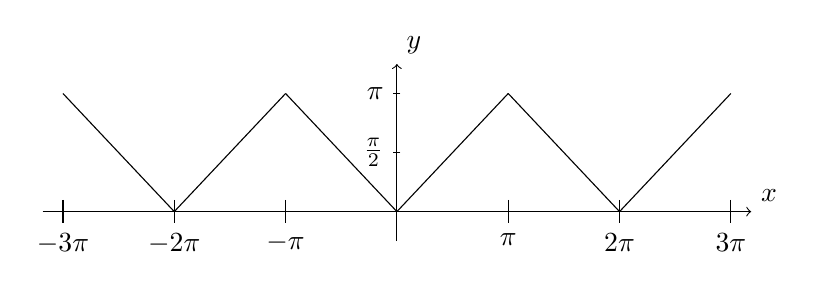
\begin{tikzpicture}[xscale=0.45,yscale=1.5]
\draw[->] (-10,0) -- (10,0) node [above right] {$x$};
\draw[->] (0,-0.25) -- (0,1.25) node [above right] {$y$}; 

% this draws all the fractional multiples of pi

%\foreach \x/\num/\den/\neg in {0.5*pi/\pi/2/,1.5*pi/3\pi/2/,-0.5*pi/\pi/2/-,-1.5*pi/3\pi/2/-} \draw ({\x},0.1) -- ({\x},-0.1) node [below] {$\neg \frac{\num}{\den}$}; 

% this draws all non fractional multiples of pi

\foreach \x/\val in {pi/\pi,2*pi/2\pi,3*pi/3\pi,-pi/-\pi,-2*pi/-2\pi,-3*pi/-3\pi} 
\draw ({\x},0.1) -- ({\x},-0.1) node [below] {$\val$}; 

\foreach \y/\val in {0.5/\frac{\pi}{2},1/\pi} \draw (0.1,\y) -- (-0.1,\y) node [left] {$\val$};

\foreach \i in {-1,0,1} {
\draw ({2*pi*\i},0) -- ({2*pi*\i+pi},1);
\draw ({2*pi*\i-pi},1) -- ({2*pi*\i},0);}

\end{tikzpicture}
\end{center}

\solution

Let $f(x)$ be the sawtooth wave defined in the picture above.  We can write it as a piecewise function as
%
\begin{align*}
f(x) & = \begin{cases}
x & 0 \leq x \leq \pi \\
-x & -\pi < x < 0 
\end{cases}
\end{align*}
and extending it periodically.  

Then using the formulas in (\ref{eq:fourier:coeff:a0})--(\ref{eq:fourier:coeff:bn}) and we will take advantage of the fact that $f(x)$ is an even function. 
%
\begin{align*}
a_0 & = \frac{1}{2\pi} \int_{-\pi}^{\pi} f(x) \, dx \\
& = \frac{2}{2\pi} \int_0^{\pi} x \,dx \\
& = \frac{1}{\pi} \frac{x^2}{2} \biggr \vert_0^{\pi} = \frac{\pi}{2}  
\end{align*}
\begin{align*}
a_n & = \frac{1}{\pi} \int_{-\pi}^{\pi} f(x) \cos nx \, dx 
\intertext{and since $\cos nx$ is even and the product of even functions is even}
 & = \frac{2}{\pi} \int_{0}^{\pi} x\cos nx \, dx 
\end{align*}
And this is a good example to use tabular integration.  

\begin{center}
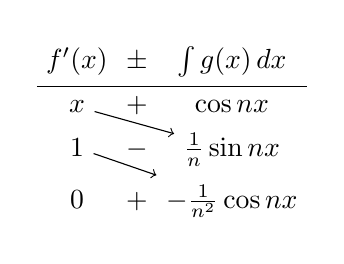
\begin{tikzpicture}[every node/.style={anchor=base}]
  \matrix
  {
    \node (f1){$f'(x)$}; & \node{$\pm$}; & \node (g1) {$\int g(x) \, dx$}; \\ \hline
    \node (f2){$x$}; & \node {$+$}; & \node (g2) {$\cos nx$}; \\
    \node (f3) {$1$}; & \node {$-$}; & \node (g3) {$\frac{1}{n} \sin nx$}; \\
    \node (f4){$0$}; & \node {$+$}; & \node (g4) {$-\frac{1}{n^2} \cos nx$}; \\
  };
    \draw[->] (f2)--(g3); 
    \draw[->] (f3)--(g4); 
\end{tikzpicture}
\end{center}
and then using the table to find
%
\begin{align*}
a_n & =\frac{2}{\pi} \biggl( \frac{x}{n} \sin nx + \frac{1}{n^2} \cos nx \biggr) \biggr \vert_0^{\pi} \\
& = \frac{2}{\pi}\biggl(\biggl(\frac{\pi}{n} \sin n \pi + \frac{1}{n^2} \cos n\pi \biggr) - 
\biggl( 0 +\frac{1}{n^2} \cos 0 \biggr) \biggr)\\
& = \frac{2}{\pi n^2} \bigl( (-1)^n - 1) 
\end{align*}

Lastly, 
%
\begin{align*}
b_n & = \frac{1}{\pi} \int_{-\pi}^{\pi} f(x) \sin nx \, dx 
\end{align*}
but this is a product of a even and an odd function, which is odd and integrating an odd function over a symmetric interval is 0.  Therefore the Fourier series is
%
\begin{align*}
F(x) & = \frac{\pi}{2} + \sum_{n=1}^{\infty} \frac{2}{\pi n^2} \bigl( (-1)^n - 1) \cos nx 
\end{align*}

\end{example}


\subsection{Convergence of a Sum of a Fourier Series} 

Since Fourier series are infinite series, it is important to consider if it converges.  As we will see, Fourier series will generally converge, to what value will depend on $x$.   Consider the Fourier series in Example \ref{ex:FS:sawtooth}.  If we let
%
\begin{align*}
F(x) & = \frac{\pi}{2} + \sum_{n=1}^{\infty} \frac{1}{n^2} \bigl( (-1)^n - 1) \cos nx
\end{align*}
we would need to text the convergence of every value of $x$.  In this case, this can be done by using the direct comparison test to the series to $\sum_{n=1}^{\infty} \frac{1}{n^2}$ which converges, so the series $F(x)$ converges for all $x$.  

This doesn't work for all series and the other difficulty is that we don't know what it converges to.  Fortunately, the following theorem gives a very nice result.  

\begin{theorem}
Let $f(x)$ be periodic with period $2\pi$ and piecewise continuous in the interval $-\pi \leq x \leq \pi$. Let $F(x)$ be the Fourier series of $f(x)$ and 
%
\begin{align*}
F(x) & = \begin{cases} f(x) & \text{if $f$ is continuous at $x$} \\
\frac{f(x^+)+f(x^-)}{2} & \text{if $f$ is not continuous at $x$}
\end{cases}
\end{align*}
In other words, the Fourier series converges to the average of the left- and right-hand limits of $f(x)$.    
\end{theorem}


\begin{example}
Show that the Fourier series of the square wave function above converges to 0 when $x=0$. 

\solution

Note that average of the left- and right-handed limits of the square wave function at $x=0$ is $(1+(-1))/2=0$, so using the theorem above, the function converges to 0 when $x=0$. 

Alternatively, we can evaluate the Fourier series of the square wave function directly.  Evaluating the Fourier series at $x=0$ is 
% 
\begin{align*}
F(0) & = \sum_{n=1}^{\infty} \frac{2}{n\pi} (1-\cos(n\pi)) \sin n x \biggl \vert_{x=0} = 0,
\end{align*}
which is consistent with that above. 

\end{example}



\subsection{Fourier Series of Functions of Period $2L$} 

We saw that the Fourier series above applied only to functions that were periodic with period $2\pi$.  This section covers functions with arbitrary periodicity, which we will call period $2L$.   If we let  $u=\frac{\pi x}{L}$, and substitute this into (\ref{eq:trig:series}), then 
% 
\begin{align}
f(x) & = a_0 + \sum_{n=1}^{\infty} \biggl( a_n \cos \frac{n\pi x}{L} + b_n \sin \frac{n \pi x}{L} \biggr)  \label{eq:FS:period:2L}
\end{align}
and then it can be shown in a similar manner to that above that (\ref{eq:fourier:coeff:a0})--(\ref{eq:fourier:coeff:bn}) can be written as
%
\begin{align}
a_0 & = \frac{1}{2L} \int_{-L}^L f(x) \, dx \label{eq:coeff:period:2L:a0} \\
a_n & = \frac{1}{L} \int_{-L}^{L} f(x) \cos \biggl( \frac{n\pi x}{L} \biggr) \, dx 
\label{eq:coeff:period:2L:an}\\
b_n & =  \frac{1}{L} \int_{-L}^{L} f(x) \sin \biggl( \frac{n\pi x}{L} \biggr) \, dx
\label{eq:coeff:period:2L:bn}
\end{align}

The series is called the Fourier series of period $2L$ with the corresponding Fourier coefficients.  


\begin{example} \label{ex:FS:x}
Find the Fourier Series of the periodic extension (of period 2) of $f(x) = x$ for $x \in [-1,1]$ as shown in the graph below:

\begin{center}
\begin{tikzpicture}
\draw[->] (-3.5,0) -- (3.5,0) node [above right] {$x$}; 
\foreach \x in {-3,-2,-1,1,2,3} \draw (\x,0.1) -- (\x,-0.1) node [below] {\x};
\draw[->] (0,-1.5) -- (0,1.5) node [above right] {$y$};
\foreach \y in {-1,1} \draw (0.1,\y) -- (-0.1,\y) node [left] {\y};

\foreach \i in {-1,0,1} \draw ({-1+2*\i},-1) -- ({1+2*\i},1); 
\end{tikzpicture}
\end{center}

\solution

To find the Fourier series, we first need to find the Fourier coefficients, by evaluating the integrals in (\ref{eq:coeff:period:2L:a0})--(\ref{eq:coeff:period:2L:bn}),

\begin{align*}
a_0  & = \frac{1}{2} \int_{-1}^1 x \, dx = 0 \intertext{because $x$ is an odd function}
a_n & = \frac{1}{1} \int_{-1}^1 x \cos n \pi x \, dx = 0 \intertext{because $x$ times $\cos n\pi x$ is odd} 
b_n & = \frac{1}{1} \int_{-1}^1 x \sin n \pi x \, dx \intertext{because $x$ times $\sin n\pi x$ is even}
& = 2\int_0^1 x \sin n\pi x \intertext{using tabular integration,}
b_n & = -\frac{x}{n\pi} \cos (n \pi x) + \frac{1}{n^2 \pi^2} \sin (n\pi x) \biggr\vert_{-1}^1 \\
& = -\frac{2}{n\pi} \cos (n\pi) = \frac{2}{n\pi} (-1)^{n+1} 
\end{align*}

The Fourier Series of the function is
% 
\begin{align*}
\sum_{n=1}^{\infty} \frac{2}{n\pi} (-1)^{n+1} \sin n \pi x  
\end{align*}
\end{example}


\section{Even and Odd Functions; Half-Range Expansions}

We saw above that the periodic extension of $f(x)=x$ on $[-1,1]$ in Example \ref{ex:FS:x} resulted in a odd function and that only the sine terms of the Fourier Series was left.  That is, all of the Fourier coefficients for the cosine terms were 0.  In this section, we use this idea to produce only even and odd extensions which results in only sine expansions or cosine expansions.  

To begin, let's clearly define an even- and odd-periodic extension.  

\begin{definition}
Let $f$ be defined on $[0,L]$ for some $L>0$.  
\begin{itemize}
\item The even periodic extension of $f$ is called $F(x)$ and is defined:
% 
\begin{align*}
F(x) & = 
\begin{cases}
f(x) & 0 \leq x \leq L \\
f(-x) &  -L \leq x < 0 \\
f(x+2kL) & \text{otherwise for appropriate integer $k$}
\end{cases}
\end{align*}
\item The odd periodic extension of $f$ is called $F(x)$ and is defined:
\begin{align*}
F(x) & =
\begin{cases}
f(x) & 0 \leq x \leq L \\
-f(-x) &  -L \leq x < 0 \\
f(x+2kL) & \text{otherwise for appropriate integer $k$}
\end{cases}
\end{align*}
\end{itemize}
\end{definition}

\begin{example}
Graph the even- and odd-periodic extension of 
% 
\begin{align*}
f(x) & = 1-x
\end{align*}
defined on $[0,1]$.  

\solution

For the even extension, we first graph the function on $[0,1]$, then make the even extension of it on $[-1,0]$.  The original function is shown below as a solid line and the even extension is dashed.

\begin{center}
\begin{tikzpicture}
\draw[->] (-3.5,0) -- (3.5,0) node [above right] {$x$}; 
\foreach \x in {-3,-2,-1,1,2,3} \draw (\x,0.1) -- (\x,-0.1) node [below] {\x};
\draw[->] (0,-1.5) -- (0,1.5) node [above right] {$y$};
\foreach \y in {-1,1} \draw (0.1,\y) -- (-0.1,\y) node [left] {\y};

\draw (0,1) -- (1,0);
\draw[dashed] (0,1) -- (-1,0);
\end{tikzpicture}
\end{center}
and then we produce the period extension of period 2. 

\begin{center}
\begin{tikzpicture}
\draw[->] (-3.5,0) -- (3.5,0) node [above right] {$x$}; 
\foreach \x in {-3,-2,-1,1,2,3} \draw (\x,0.1) -- (\x,-0.1) node [below] {\x};
\draw[->] (0,-1.5) -- (0,1.5) node [above right] {$y$};
\foreach \y in {-1,1} \draw (0.1,\y) -- (-0.1,\y) node [left] {\y};

\foreach \i in {-1,0,1} \draw ({-1+2*\i},0) -- ({2*\i},1) -- ({1+2*\i},0); 
\draw[->] (3,0) -- (3.5,0.5);
\draw[<-] (-3.5,0.5) -- (-3,0); 
\end{tikzpicture}
\end{center}

To find the odd extension, flip the original function on $[0,1]$ around the origin to get:

\begin{center}
\begin{tikzpicture}
\draw[->] (-3.5,0) -- (3.5,0) node [above right] {$x$}; 
\foreach \x in {-3,-2,-1,1,2,3} \draw (\x,0.1) -- (\x,-0.1) node [below] {\x};
\draw[->] (0,-1.5) -- (0,1.5) node [above right] {$y$};
\foreach \y in {-1,1} \draw (0.1,\y) -- (-0.1,\y) node [left] {\y};

\draw (0,1) -- (1,0);
\draw[dashed] (0,-1) -- (-1,0);
\end{tikzpicture}
\end{center}

Then extend the function on $[-1,1]$ in a periodic way.  

\begin{center}
\begin{tikzpicture}
\draw[->] (-3.5,0) -- (3.5,0) node [above right] {$x$}; 
\foreach \x in {-3,-2,-1,1,2,3} \draw (\x,0.1) -- (\x,-0.1) node [below] {\x};
\draw[->] (0,-1.5) -- (0,1.5) node [above right] {$y$};
\foreach \y in {-1,1} \draw (0.1,\y) -- (-0.1,\y) node [left] {\y};

\foreach \i in {-2,-1,0,1} \draw ({2*\i},1) -- ({2+2*\i},-1); 
\end{tikzpicture}
\end{center}


\end{example}


\subsection{The Fourier Sine and Cosine Series}

We now address the Fourier series of the even- and odd-periodic extensions of $f$ on $[0,L]$.  As in Example \ref{ex:FS:x}, there are no cosine terms and the Fourier series of the odd periodic extension of $f$ can be written 
% 
\begin{align} 
f(x) & = \sum_{n=1}^{\infty} b_n \sin \biggl(\frac{n\pi x}{L} \biggr) \label{eq:FS:sine}
\intertext{where,}
b_n & = \frac{2}{L} \int_{0}^L f(x) \sin \biggl(\frac{n\pi x}{L} \biggr) \,dx  \label{eq:FS:sine:bn}
\end{align}
and this is often called the \textbf{Fourier sine series}.\index{Fourier sine series}  

Similarly, the Fourier series of the even periodic extension of $f$ is
% 
\begin{align}
f(x) &= a_0 + \sum_{n=1}^{\infty} a_n \cos \biggl( \frac{n \pi x}{L} \biggr) \label{eq:FS:cosine}
\intertext{where}
a_0 & = \frac{1}{L} \int_{0}^L f(x) \, dx \label{eq:FS:cosine:a0}\\
a_n & = \frac{2}{L} \int_0^L f(x) \cos \biggl( \frac{n\pi x}{L} \biggr)\, dx \label{eq:FS:cosine:an}
\end{align}
and is called the \textbf{Fourier cosine series}.\index{Fourier cosine series}


\begin{example}
Find the Fourier Cosine Series of $f(x) = x$ for $0 \leq x \leq 1$. 

\solution

For this, we need to find the coefficients in (\ref{eq:FS:cosine:a0}) and (\ref{eq:FS:cosine:an}),
\begin{align*}
a_0 & = \frac{1}{1} \int_0^1 x \,dx = \frac{1}{2} \\
a_n & = \frac{2}{1} \int_0^1 x \cos n \pi x \, dx \\
& = \frac{2(\cos n\pi -1)}{n \pi} = \frac{2}{n\pi} \bigl((-1)^n-1\bigr) 
\end{align*}
and use (\ref{eq:FS:cosine}) to find 
% 
\begin{align*}
f(x) & = \frac{1}{2} + \sum_{n=1}^{\infty} \frac{2}{n\pi} \bigl((-1)^n-1\bigr)  \cos n \pi x 
\end{align*}
\end{example}

\phantom{hi}

\begin{example}
Find the odd periodic extension of $f(x) = x^2$ on $[0,2]$.   A graph of this is:

\begin{center}
\begin{tikzpicture}[xscale=0.75,yscale=0.5]
\draw[->] (-6.5,0) -- (6.5,0) node [above right] {$x$}; 
\foreach \x in {-6,-5,...,-1,1,2,...,6} \draw (\x,0.1) -- (\x,-0.1) node [below] {\x};
\draw[->] (0,-4.5) -- (0,4.5) node [above right] {$y$};
\foreach \y in {-4,-3,-2,-1,1,2,3,4} \draw (0.1,\y) -- (-0.1,\y) node [left] {\y};

\foreach \i in {-1,0,1} {
\draw plot[domain={4*\i+0}:{4*\i+2}] (\x,{(\x-4*\i)*(\x-4*\i)});
\draw plot[domain={4*\i-2}:{4*\i+0}] (\x,{-1*(\x-4*\i)*(\x-4*\i)});
}
\end{tikzpicture}
\end{center}

\solution

For this, we need to find $b_n$ from (\ref{eq:FS:sine:bn}),
%
\begin{align*}
b_n & = \frac{2}{2} \int_0^2 x^2 \sin \biggl( \frac{n \pi x}{2} \biggr)  \, dx 
\intertext{and again, this can be done using tabular integration,}
& = -\frac{2 \, x^{2}}{n \pi} \cos \biggl( \frac{n \pi x}{2} \biggr) +
\frac{8 \, x}{n^2\pi^2}  \sin \biggl( \frac{n \pi x}{2} \biggr) +
\frac{16}{n^3\pi^3} \cos \biggl( \frac{n \pi x}{2} \biggr)
 \biggr \vert_0^2 \\
& = -\frac{8}{n \pi} \cos (n \pi) + \frac{16}{n^3\pi^3} \cos (n \pi)  = \frac{16-8n^2\pi^2}{n^3 \pi^3} (-1)^n 
\end{align*}
and then use this in (\ref{eq:FS:sine})
%
\begin{align*}
f(x) & = \sum_{n=1}^{\infty}\frac{16-8n^2\pi^2}{n^3 \pi^3} (-1)^n  \sin \biggl(\frac{n \pi x}{2} \biggr) 
\end{align*}

\end{example}


\section{Approximation by Trigonometric Polynomials}

Consider a periodic function $f$ of period $2\pi$ on the interval $[-\pi,\pi]$.  
The $N$th partial sum of the Fourier Series of $f$ is denoted $f_N$, 

\begin{align*}
f_N(x) & = a_0 + \sum_{n=1}^N (a_n \cos nx + b_n \sin nx)
\end{align*}
where $a_0, a_n$ and $b_n$ are the Fourier Coefficients as before.  The function $f_N$ is also called the \textbf{Trigonometric Polynomial of degree $n$}. \index{trigonometry polynomial}

Let's ask a question about approximation.  Consider a function of the form:
% 
\begin{align*}
F_N(x) & =A_0 + \sum_{n=1}^N (A_n \cos nx + B_n \sin nx)
\end{align*}
What is the best approximate for a trigonometric polynomial to another function $F(x)$.  That is, what coefficients can be chosen $A_0, A_n, B_n$? 

To answer this question, we will need to know what error we are taking about.  Typically the error will be some function of the two functions, called $E(f,g)$ that outputs a number.  We would like the error to have the following properties:
\begin{align*}
E(f,g) & = E(g,f) \\
E(f,g) & \geq 0 \\
E(f,f) & = 0 
\end{align*}
one such function that we know is the square of the function norm or 
%
\begin{align*}
E(F,F_N) & = \langle F-F_N,F-F_N \rangle = ||F-F_N||^2   \\
& = \int_{-\pi}^{\pi} (F(x)-F_N(x))^2 \, dx \\
& = \int_{-\pi}^{\pi}\bigl(F(x) - A_0 - \sum_{n=1}^{N} (A_n \cos nx + B_n \sin nx) \bigr)^2
\end{align*}

To find the minimum of this, we will take the derivatives of $E$ with respect to $A_0, A_n$ and $B_n$:

\begin{align*}
\frac{\partial E}{\partial A_0} & = -2 \int_{-\pi}^{\pi} \bigl(F(x) - A_0 - \sum_{n=1}^{N} (A_n \cos nx + B_n \sin nx ) \bigr)  \\
0 & = \langle F, 1\rangle - \langle A_0, 1 \rangle - \sum_{n=1}^{N} (\langle A_n \cos n x, 1 \rangle + \langle B_n \sin nx, 1 \rangle )  \\
0 & = \langle F, 1\rangle - A_0\langle 1, 1 \rangle  \intertext{or}
A_0 & = \frac{\langle F,1\rangle}{\langle 1,1 \rangle} = \frac{1}{2\pi} \int_{-\pi}^{\pi} F(x)\,dx 
\end{align*}

Similarly take the derivative with respect to $A_m$:

\begin{align*}
\frac{\partial E}{\partial A_m} & = -2 \int_{-\pi}^{\pi} \cos mx \bigl(F(x) - A_0 - \sum_{n=1}^{N} (A_n \cos nx + B_n \sin nx ) \bigr)  \intertext{set the derivative to 0} 
0 & = \langle F, \cos mx \rangle - \langle A_0, \cos  mx \rangle \\
& \qquad - \sum_{n=1}^{N} (\langle A_n \cos n x, \cos mx \rangle + \langle B_n \sin nx, \cos mx \rangle )  
\intertext{Note that $\langle \cos nx,\cos mx\rangle =0$ unless $m=n$ and $\langle 1,\cos mx\rangle=0$} 
0 & = \langle F, \cos mx \rangle - A_m \langle \cos mx, \cos mx \rangle  \intertext{or}
A_m & = \frac{\langle F, \cos mx\rangle }{\langle \cos mx, \cos mx \rangle } \\
& = \frac{1}{\pi} \int_{-\pi}^{\pi} F(x) \cos m x \, dx 
\end{align*}

And similarly it can be shown that 
% 
\begin{align*}
B_m & = \frac{1}{\pi} \int_{-\pi}^{\pi} F(x) \sin mx \, dx 
\end{align*}


\begin{Boxed*}
Let $f(x)$ be a piecewise continuous function on $[-\pi,\pi]$, $N>0$ and 
%
\begin{align*}
f_N (x) & =  a_0 + \sum_{n=1}^N (a_n \cos nx + b_n \sin nx)
\end{align*}
The values of $a_n$ and $b_n$ that minimize $||f-f_N||$ (or $||f-f_N||^2$) is
%
\begin{align*}
a_0 & = \frac{1}{2\pi} \int_{-\pi}^{\pi} f(x) \, dx \\
a_n & = \frac{1}{\pi} \int_{-\pi}^{\pi} f(x) \cos n x \, dx \\
b_n & = \frac{1}{\pi} \int_{-\pi}^{\pi} f(x) \sin n x \, dx \\
\end{align*}
that is they are the Fourier Coefficients.  
\end{Boxed*}

\phantom{hi}

\begin{example}
In Example \ref{ex:FS:sawtooth}, the Fourier series of the sawtooth function was found the Fourier Coefficients are:
\begin{align*}
a_0 & = \frac{\pi}{2} \\
a_n & = \frac{2}{\pi n^2} ((-1)^n-1) \qquad \text{$n\geq 1$} \\
b_n & = 0 
\end{align*}

Graph the sawtooth function and $f_{9}(x)$, the $9$th degree trigonometric polynomial.  

\solution

 \begin{center}
\begin{tikzpicture}[xscale=0.45,yscale=0.75]
\draw[->] (-10,0) -- (10,0) node [above right] {$x$};
\draw[->] (0,-0.25) -- (0,3.5) node [above right] {$y$}; 

% this draws all the fractional multiples of pi

%\foreach \x/\num/\den/\neg in {0.5*pi/\pi/2/,1.5*pi/3\pi/2/,-0.5*pi/\pi/2/-,-1.5*pi/3\pi/2/-} \draw ({\x},0.1) -- ({\x},-0.1) node [below] {$\neg \frac{\num}{\den}$}; 

% this draws all non fractional multiples of pi

\foreach \x/\val in {pi/\pi,2*pi/2\pi,3*pi/3\pi,-pi/-\pi,-2*pi/-2\pi,-3*pi/-3\pi} 
\draw ({\x},0.1) -- ({\x},-0.1) node [below] {$\val$}; 

\foreach \y/\val in {0.5*pi/\frac{\pi}{2},pi/\pi} \draw (0.1,\y) -- (-0.1,\y) node [left] {$\val$};

\foreach \i in {-1,0,1} {
\draw ({2*pi*\i},0) -- ({2*pi*\i+pi},{pi});
\draw ({2*pi*\i-pi},{pi}) -- ({2*pi*\i},0);}
%
%\draw plot[domain=-10:10,samples=250] (\x,{pi/2+4/pi*(-263/315*cos(\x r)+656/945*pow(cos(\x r),3)-1936/525*pow(cos(\x r),5)+2560/441*pow(cos(\x r),7)-256/81*pow(cos(\x r),9))});
%
\begin{luacode}
local function wave(x)
    sum = math.pi*0.5
	for n = 1, 9, 2 do
 	   sum = sum - 4*math.cos(n*x)/(math.pi*n*n)
    end
    return sum
end

local xmin = -10
local xmax = 10 
local x = xmin
local numpoints = 500
local y 
tex.print('\\draw[color=red]')
for i = 0,numpoints-1 do
    y = wave(x)
    tex.print('(',x,',',y,') -- ')
    x = x + (xmax-xmin)/numpoints
end
tex.print('(',x,',',y,');')

\end{luacode}




\end{tikzpicture}
\end{center}

and the two plots are indistinguishable on this scale.  


\end{example}

\begin{example} \label{ex:plot:square:wave}
In Example \ref{ex:FS:square:wave}, the Fourier series of the square wave function was found and the Fourier Coefficients are:
\begin{align*}
a_0 & = 0 \\
a_n & = 0 \\
b_n & =  \frac{2}{n\pi} (1- (-1)^n) 
\end{align*}

Graph the square wave function and $f_{9}(x)$, the $9$th degree trigonometric polynomial.  

\solution

\begin{center}
\begin{tikzpicture}[xscale=0.45,yscale=1.5]
\draw[->] (-10,0) -- (10,0) node [above right] {$x$};
\draw[->] (0,-1.25) -- (0,1.25) node [above right] {$y$}; 

% this draws all non fractional multiples of pi

\foreach \x/\val in {pi/\pi,2*pi/2\pi,3*pi/3\pi,-pi/-\pi,-2*pi/-2\pi,-3*pi/-3\pi} 
\draw ({\x},0.1) -- ({\x},-0.1) node [below] {$\val$}; 

\foreach \y in {-1,1} \draw (0.1,\y) -- (-0.1,\y) node [left] {\y};

\foreach \i in {-1,0,1} {
\draw ({2*pi*\i},1) -- ({2*pi*\i+pi},1);
\draw ({2*pi*\i-pi},-1) -- ({2*pi*\i},-1);}


\begin{luacode}
local function wave(x)
    sum = 0.0
	for n = 1, 9, 2 do
 	   sum = sum + math.sin(n*x)/n
    end
    return sum*4/math.pi
end

local xmin = -10
local xmax = 10 
local x = xmin
local numpoints = 500
local y 
tex.print('\\draw[color=red]')
for i = 0,numpoints-1 do
    y = wave(x)
    tex.print('(',x,',',y,') -- ')
    x = x + (xmax-xmin)/numpoints
end
tex.print('(',x,',',y,');')

\end{luacode}


\end{tikzpicture}
\end{center}

And in contrast to the previous example, the trigonometric polynomial $f_9(x)$ and the original function $f$ are quite different.  


\end{example}

We will explore this example in a bit more detail after seeing some important theorems. 


\subsection{Theorems Related to Fourier Series}

\begin{theorem}
The quantity $||F-F_N||^2$ on the interval $[-\pi,\pi]$ is the minimum if and only if the coefficients of $F_N$ in (2) ar the Fourier coefficients of $F$.  This minimum value is 
% 
\begin{align} \label{eq:Estar}
E^{\star} & = \int_{-\pi}^{\pi} f^2 \, dx - 2A_0\pi - \pi \sum_{n=1}^{N} (A_n^2 + B_n^2) 
\end{align}
\end{theorem}

\begin{theorem}[Bessel's Inequality]
Let $a_0, a_n$ and $b_n$ be the fourier coefficients related to the function $f$ on $[-\pi,\pi]$. Then
\begin{align*}
2a_0^2 + \sum_{n=1}^N (a_n^2+b_n^2) \leq \frac{1}{\pi} \int_{-\pi}^{\pi} f^2 \, dx 
\end{align*}
\end{theorem}

\begin{theorem}[Parseval's Theorem]
Let $a_0, a_n$ and $b_n$ be the fourier coefficients related to the function $f$ on $[-\pi,\pi]$. Then
\begin{align*}
2a_0^2 + \sum_{n=1}^{\infty} (a_n^2+b_n^2) = \frac{1}{\pi} \int_{-\pi}^{\pi} f^2 \, dx 
\end{align*}

\end{theorem}

There are two important consequences of this theorem:

\begin{itemize}
\item If the integral on the right side is finite, then the series on the left converges.   Functions in which the right side is finite are piecewise continuous functions.

\item The error, $E^{\star}$ in (\ref{eq:Estar}) goes to zero.  That is Fourier Series converge to $f$ (using the square error).  
\end{itemize}

\begin{example}
 Calculate $E^{\star}$ for the function:
 % 
 \begin{align*}
f(x) & = \begin{cases}
\pi+x & x \in [-\pi,0) \\
\pi-x & x \in [0,\pi]  
\end{cases}
\end{align*}
and extended periodically and let $N=5,10,25,50,100,250,500,1000$.  

\solution

The Fourier Series of this function is 
% 
\begin{align*}
f(x) & = \frac{\pi}{2} + \sum_{n=1}^{\infty} \frac{2}{\pi n^2} (1-(-1)^n) \cos nx 
\end{align*}

or $a_0 = \pi/2$ and $a_n = (2/\pi n^2)(1-(-1)^n) $

\begin{align*}
E^{\star} & = \int_{-\pi}^{\pi} f^2 \, dx - 2A_0\pi - \pi \sum_{n=1}^{N} (A_n^2 + B_n^2)  \\
& = 2\int_{0}^{\pi} (\pi-x)^2 \, dx - 2\biggl(\frac{\pi}{2}\biggr) - \pi \sum_{n=1}^{N}\biggl(\frac{2}{\pi n^2} (1-(-1)^n) \biggr) 
\end{align*}

\begin{tabular}{l|l}
$n$ & $E^{\star}$ \\ \hline
5 & 0.00372 \\
10 & 0.000832 \\
25 & 0.0000482 \\
50 & $6.78 \times 10^{-6} $ \\
100 & $8.49 \times 10^{-8} $ \\
250 & $ 5.43 \times 10^{-8} $ \\
500 & $6.79 \times 10^{-9} $ \\
1000 & $8.48 \times 10^{-10} $ 
\end{tabular}

\end{example}

A consequence of Parseval's Theorem is that for piecewise continuous functions, the Fourier Series converges as $n \rightarrow \infty$.  So in light of the plot in Example \ref{ex:plot:square:wave}, that it would appear that the plot of $f_N$ would approach the square wave as $N \rightarrow \infty$.  However the plots of $f_{25}$ and $f_{100}$ are shown below (with $n=25$ on top):


\begin{center}
\begin{tikzpicture}[xscale=0.45,yscale=1.5]
\draw[->] (-10,0) -- (10,0) node [above right] {$x$};
\draw[->] (0,-1.25) -- (0,1.25) node [above right] {$y$}; 

% this draws all non fractional multiples of pi

\foreach \x/\val in {pi/\pi,2*pi/2\pi,3*pi/3\pi,-pi/-\pi,-2*pi/-2\pi,-3*pi/-3\pi} 
\draw ({\x},0.1) -- ({\x},-0.1) node [below] {$\val$}; 

\foreach \y in {-1,1} \draw (0.1,\y) -- (-0.1,\y) node [left] {\y};

\foreach \i in {-1,0,1} {
\draw ({2*pi*\i},1) -- ({2*pi*\i+pi},1);
\draw ({2*pi*\i-pi},-1) -- ({2*pi*\i},-1);}

\begin{luacode}
local function wave(x)
    sum = 0.0
	for n = 1, 25, 2 do
 	   sum = sum + math.sin(n*x)/n
    end
    return sum*4/math.pi
end

local x = -10
local numpoints = 250
local y 
tex.print('\\draw[color=red]')
for i = 0,numpoints-1,1 do
    y = wave(x)
    tex.print('(',x,',',y,') -- ')
    x = x + 20/numpoints
end
tex.print('(',x,',',y,');')

\end{luacode}

\end{tikzpicture}
\end{center}

\begin{center}
\begin{tikzpicture}[xscale=0.45,yscale=1.5]
\draw[->] (-10,0) -- (10,0) node [above right] {$x$};
\draw[->] (0,-1.25) -- (0,1.25) node [above right] {$y$}; 

% this draws all non fractional multiples of pi

\foreach \x/\val in {pi/\pi,2*pi/2\pi,3*pi/3\pi,-pi/-\pi,-2*pi/-2\pi,-3*pi/-3\pi} 
\draw ({\x},0.1) -- ({\x},-0.1) node [below] {$\val$}; 

\foreach \y in {-1,1} \draw (0.1,\y) -- (-0.1,\y) node [left] {\y};

\foreach \i in {-1,0,1} {
\draw ({2*pi*\i},1) -- ({2*pi*\i+pi},1);
\draw ({2*pi*\i-pi},-1) -- ({2*pi*\i},-1);}

\begin{luacode}
local function wave(x)
    sum = 0.0
	for n = 1, 100, 2 do
 	   sum = sum + math.sin(n*x)/n
    end
    return sum*4/math.pi
end

local x = -10
local numpoints = 250
local y 
tex.print('\\draw[color=red]')
for i = 0,numpoints-1,1 do
    y = wave(x)
    tex.print('(',x,',',y,') -- ')
    x = x + 20/numpoints
end
tex.print('(',x,',',y,');')

\end{luacode}

\end{tikzpicture}
\end{center}


And despite the larger value of $N$, $f_N$ does not appear to be approaching the square wave function.  The difference is pronounced near the discontinuities in the function.  This is called \emph{Gibbs Phenomena} and it can be shown in this situation that the local max near $x=0$ in fact grows without bound as $N \rightarrow \infty$, despite the fact that $||f_N-f|| \rightarrow 0$.  

\section{The Fourier Series using the complex exponential}

Recall that the Fourier Series of $f(x)$ on $[-\pi,\pi]$ is
%
\begin{align*}
f(x) & = a_0 + \sum_{n=1}^{\infty} (a_n \cos n x + b_n \sin n x)
\end{align*}
where 
%
\begin{align*}
a_0 & = \frac{\langle f,1 \rangle}{\langle 1,1 \rangle} = \frac{1}{2\pi} \int_{-\pi}^{\pi} f(x) \,dx \\
a_n & = \frac{\langle f, \cos nx \rangle}{\langle \cos nx, \cos nx \rangle} = \frac{1}{\pi} \int_{-\pi}^{\pi} f(x) \cos nx \,dx \\
b_n & =\frac{\langle f,\sin nx \rangle}{\langle \sin nx, \sin nx \rangle} =  \frac{1}{\pi} \int_{-\pi}^{\pi} f(x) \sin n x \,dx \\
\end{align*}
and if $f(x)$ is a real-valued function then $a_0, a_n$ and $b_n$ are real values. 

If we use the identities:
%
\begin{align*}
\cos nx & = \frac{1}{2} ( e^{inx} + e^{-inx}) \\
\sin nx & = \frac{1}{2i} (e^{inx} - e^{-inx})
\end{align*}
then the Fourier Series can be written:
%
\begin{align*}
f(x) & = a_0 + \sum_{n=1}^{\infty} (\frac{a_n}{2} ( e^{inx} + e^{-inx}) + \frac{b_n}{2i} (e^{inx} - e^{-inx}) \\
& = a_0 + \frac{1}{2} \sum_{n=1}^{\infty} (a_n-ib_n) e^{inx}  + (a_n + ib_n) e^{-inx}  
\end{align*}
if we let $c_0=a_0$ and $c_n = (a_n-ib_n)/2$ for $n>0$ and $c_n=(a_{-n} + ib_{-n})$ for $n<0$ then we can write the sum as
%
\begin{align*}
f(x) & = c_0 + \sum_{n=1}^{\infty} c_n e^{inx} + c_{-n} e^{-inx} \\
& = \sum_{n=-\infty}^{\infty} c_n e^{inx}  
\end{align*}
where
%
\begin{align*}
c_0 & = \frac{1}{2\pi} \int_{-\pi}^{\pi} f(x) \, dx \\
c_n & = \frac{a_n-ib_n}{2} = \frac{1}{2}\cdot \frac{1}{\pi} \int_{-\pi}^{\pi} f(x) (\cos nx -i \sin nx) \, dx \\
& = \frac{1}{2\pi} \int_{-\pi}^{\pi} f(x) e^{-inx} \, dx \\
c_{-n} & = \frac{a_n+ib_n}{2} = \frac{1}{2}\cdot \frac{1}{\pi} \int_{-\pi}^{\pi} f(x) (\cos nx +i \sin nx) \, dx \\
& = \frac{1}{2\pi} \int_{-\pi}^{\pi} f(x) e^{inx} \, dx \\
\end{align*}
and since $c_{-n}$ is consistent with $c_n$, we use $c_n$ for all $n \neq 0$ and actually since that is also consistent, then 
%
\begin{align*}
c_n & = \frac{1}{2\pi} \int_{-\pi}^{\pi} f(x) e^{-inx} \, dx \\
\end{align*}

If we take the interval from $[-L,L]$ instead of from $[-\pi,\pi]$ we get 
%
\begin{align*}
f(x) & = \sum_{n=-\infty}^{\infty} c_n e^{2\pi i x/L} \intertext{where}
c_n & = \frac{1}{2L} \int_{-L}^{L} f(x) e^{-2\pi i x/L} 
\end{align*}

\begin{example}
Find the complex Fourier series on $[-\pi,\pi]$ if $f(x)=x$.  

\solution
\begin{align*}
c_n & = \frac{1}{2\pi} \int_{-\pi}^{\pi} x e^{-inx} \, dx \\
& = \begin{cases}
0 & n= 0 \\
\frac{-2i\pi}{n} e^{-i \pi n}=\frac{-2(-1)^n\pi}{n}   & \text{otherwise} 
\end{cases}
\end{align*}
\end{example}

As you can see, finding the complex Fourier Series is generally easier in terms of only needing to find one integral instead of 3 for the standard Fourier Series.  



